\section{Design Concepts}
\label{sec:design}

Our approach to support the design of self-adaptive CPS software is
intentionally simple. However, the lack of a principled approach in
this domain is currently hampering the field at
large~\cite{Picco:2010:SEW:1882362.1882421}. % Key in our
% approach is the combination of design-time support and programming
% model. We illustrate the latter in Section~\ref{sec:conesc}.

We define two key design concepts: \emph{i)} individual
\emph{contexts}; and \emph{ii)} \emph{context groups}, along with the
notions necessary to weave these concepts into a complete design.
Contexts represent the different environmental situations the system
may encounter, and correspond to behavioral variations associated to a
given situation. As the environment surrounding the system mutates,
the software adapts accordingly by \emph{activating} a suitable
context. Context groups represent collections of individual contexts
sharing common characteristics; e.g., whenever the \emph{same}
functionality must adapt to changes in the surrounding environment.

\begin{figure}
\begin{center}
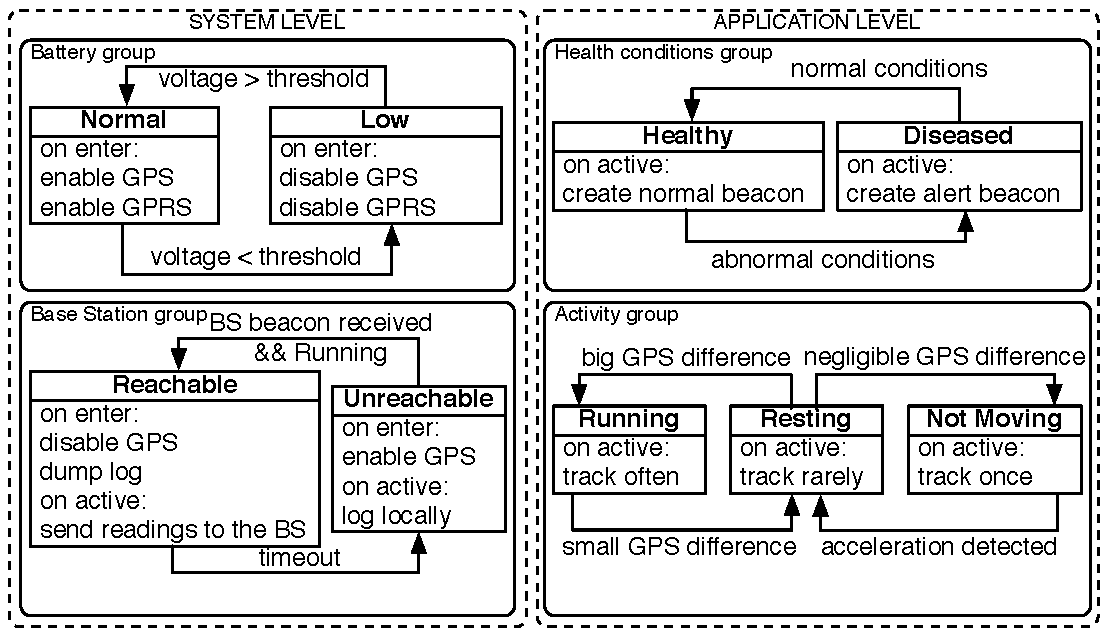
\includegraphics[scale=.45]{imgs/wildlifetracking}
\vspace{-4mm}
\caption{Wildlife monitoring application design.}
  \label{fig:design}
\vspace{-6mm}
\end{center}
\end{figure}

As n example, Figure~\ref{fig:design} graphically depicts the
context-oriented design of the wildlife monitoring applications
described earlier. Context groups are defined to describe behavioral
variations corresponding to battery levels, base-station reachability,
as well as an animal's health conditions and activity. Context groups
are tagged as system-level or application-level to discern
application-specific functionality from likely re-usable system
services.

The contexts within a group define the individual behavioral
variations. For example, the software must behave differently
depending on whether the base-station is reachable.  The contexts in a
group are tied with explicit \emph{transitions}, labeled with the
conditions triggering the context change. For example, within the
``Base-station'' group, the system transitions from context
``Reachable'' to ``Unreachable'' whenever no beacons are received from
the base-station within a specific timeout. This entails a node is out
of the base-station radio range and the software must adapt
accordingly; for example, by locally storing the contact logs instead
of sending them over the radio.

The specific software adaptation is encapsulated in the individual
contexts. In the latter, it is useful to distinguish between \emph{one-time
  operations} executed at the time of entering or existing a context,
and \emph{continuous activities} that occur as long as a context is
active. For example, on entering context ``Reachable'', the software
dumps on the base-station the contact logs locally accumulated while
the latter was unreachable. Similarly, when in the latter situation,
the software must log the contacts locally as long as the
``Unreachable'' context persists, as shown in Figure~\ref{fig:design}.

The required adaptation functionality may span multiple context
groups. To this end, developers can bind context activations across
groups. An example is in the ``Reachable'' context within the
``Base-station'' group: on entering, context ``NotMoving'' should
also consequently activate. As base-stations are typically deployed at
known locations, and yet their radio range is very limited, continuing
to sample the GPS sensor is likely a waste of energy, as a node's
locations can be approximated with the base-station one. Hence we can
avoid waiting for the next GPS sample before deciding to stop
sampling until an acceleration is detected.

Developers may also make context transitions subject to the activation
of other contexts, which is useful to check for design errors at
run-time. An example is when activating the ``Diseased'' context in
the ``Health conditions'' group. Besides an abnormal body temperature
that may reveal a disease, the adaptation process must check that
either ``Resting'' or ``NotMoving'' in the ``Animal activity'' group
is currently active. Indeed, if an animal is diseased, it is probably
not very active. Should that not be the case, developers might have
not correctly captured how contexts evolve, potentially indicating a
design error.

The concepts we define provide design-time support to reason on the
different situations the software must adapt to, and to identify common
functionality, orthogonal aspects, and mutual constraints. This
ultimately helps separate concerns during the implementation phase, as
we illustrate next.



%%% Local Variables: 
%%% mode: latex
%%% TeX-master: "paper"
%%% End: 
